\subsection{Ca sử dụng tạo video recap}

\vspace{0.2cm}

\noindent 
\begin{tabularx}{\linewidth}{| l | X |} 
\hline 
\textbf{Mô tả} & Người dùng tạo video recap từ các ảnh trong thư viện. \\
\hline 
\textbf{Luồng cơ bản} & 1. Người dùng bấm nút tạo video recap từ thanh công cụ ở dưới màn hình. \newline
                       2. Hệ thống hiển thị giao diện chọn danh sách ảnh.\newline
                       3. Người dùng chọn ảnh trong danh sách ảnh đã tải lên hệ thống. \newline
                       4. Người dùng chọn ảnh trong danh sách ảnh của máy người dùng.\newline
                       5. Người dùng bấm submit danh sách ảnh. \newline
                       6. Hệ thống tạo kịch bản cho video và những tùy chỉnh mặc định cho video từ danh sách ảnh: style khung ảnh, nhạc nền, chất lượng video, thời lượng video, chủ đề video. \newline
                       7. Người dùng chỉnh các tùy chỉnh cho video: style khung ảnh, nhạc nền, chất lượng video, thời lượng video, chủ đề video. \newline
                       8. Người dùng bấm submit để tạo video. \newline
                       9. Hệ thống tạo video từ danh sách ảnh và kịch bản đã chọn. \newline
                       10. Hệ thống điều hướng đến màn hình xem trạng thái tạo video theo thời gian thực. \\
\hline 
\textbf{Tiền điều kiện} & - Người dùng đã đăng nhập vào hệ thống. \newline
                            - Người dùng đã có ảnh trong thư viện. \\
\hline
\textbf{Hậu điều kiện} & - Hệ thống hiển thị trạng thái và tiến độ tạo video theo thời gian thực. \newline
                         - Người dùng quay về màn hình danh sách video để theo dõi trạng thái video đã tạo. \\
\hline 
\textbf{Yêu cầu phi chức năng} & - Hệ thống xử lý tạo kịch bản video không quá 20s. \newline 
                                 - Hệ thống tạo video không quá 5 phút. \newline
                                 - Hệ thống cập nhật trạng thái video theo thời gian thực. \\
\hline 
\end{tabularx}

\vspace{0.8cm}

\noindent 
\begin{tabular}{| c | c |}
    \hline
    \textbf{Biểu đồ hoạt động} & \textbf{Quan hệ} \\ 
    \hline
    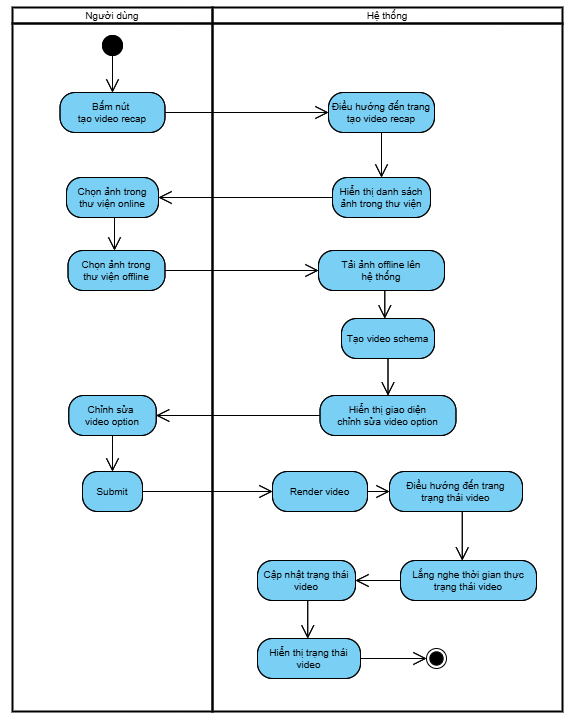
\includegraphics[width=0.6\linewidth]{figures/c3/3-3-9-activity-diagram.png} 
    &  
    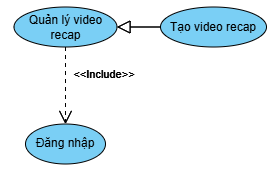
\includegraphics[width=0.35\linewidth]{figures/c3/3-3-9-relationship.png} \\ 
    \hline
\end{tabular}

\begin{figure}[H]
    \centering  
    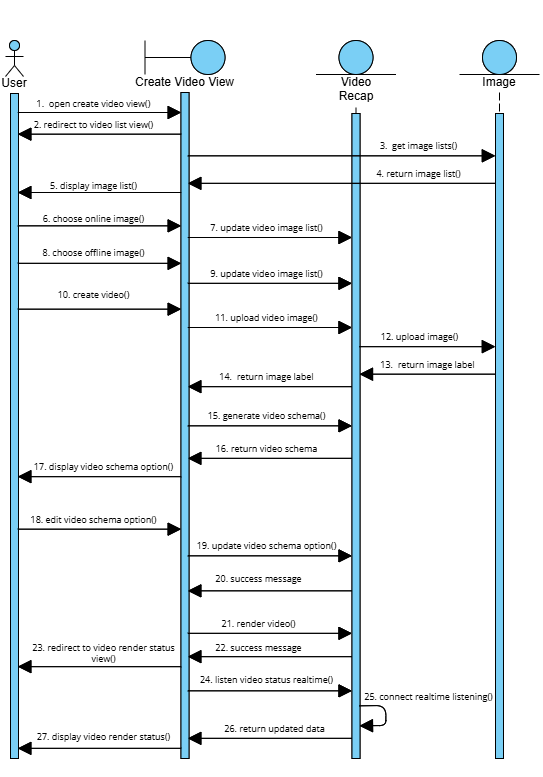
\includegraphics[width=1.1\textwidth]{figures/c3/3-3-9-sequence-diagram.png}
    \caption{Biểu đồ tuần tự ca sử dụng tạo video recap.}
    \label{fig:3-3-9-sequence-diagram}
\end{figure}
